% 0212(본책 42쪽) — △ABC(AB=6, AC=4), 변의 길이는 파선 호로 표시. 스캔 삽화를 TikZ 로 다시 그림. 답(넓이)·∠A 는 적지 않는다.
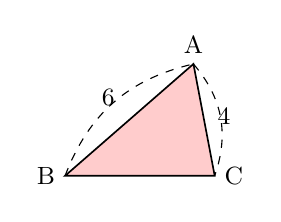
\begin{tikzpicture}[line width=0.6pt]
  \coordinate (B) at (0,0); \coordinate (C) at (1.9,0); \coordinate (A) at (1.63,1.42);
  \fill[red!20] (A) -- (B) -- (C) -- cycle;
  \draw (A) -- (B) -- (C) -- cycle;
  \draw[dashed, line width=0.4pt] (B) to[bend left=28] (A);
  \node[font=\small] at (0.55,1.0) {$6$};
  \draw[dashed, line width=0.4pt] (A) to[bend left=30] (C);
  \node[font=\small] at (2.02,0.75) {$4$};
  \node[font=\small, above] at (A) {A};
  \node[font=\small, left] at (B) {B};
  \node[font=\small, right] at (C) {C};
\end{tikzpicture}
